\documentclass[a4paper,12pt]{article}
\usepackage[utf8]{inputenc}
\usepackage[spanish]{babel}
\usepackage{graphicx}
\usepackage{amsmath}
\usepackage{booktabs}
\usepackage{hyperref}
\usepackage{geometry}
\geometry{margin=2.5cm}

\title{\texttt{Simulación de un Bot de Trading \\usando Eventos Discretos}}
\author{\\Darío López Falcón \\ Universidad de la Habana (UH) \\ Facultad de Matemática 
y Computación (MATCOM)}
\date{\today}

\begin{document}

\maketitle

\section*{S1. Introducción}

Este proyecto tiene como objetivo simular y analizar el comportamiento de un bot de trading 
usando técnicas de simulación de eventos discretos. Se busca evaluar cómo diferentes 
configuraciones del bot responden bajo distintos escenarios de mercado simulados estocásticamente. 
A partir de esto, se pretende aplicar herramientas estadísticas reales para realizar comparaciones, 
validar hipótesis y explorar el impacto de variables como la volatilidad del mercado, el horizonte 
temporal y la estrategia del bot.\\

\textbf{Variables de interés:} ganancia neta, cantidad de operaciones realizadas, 
valor final del portafolio, umbrales de compra y venta, comisión por transacción.

%%AGREGAR TABLA DE BOTS Y PARAMETROS USADOS

\section*{S2. Detalles de Implementación}

\subsection*{Simulación del sistema}
La simulación se implementó en Python, usando una arquitectura modular.\\

\textbf{Estructura modular del código:}
\begin{itemize}
\item \texttt{main.py}: ejemplo simple de simulacion, sin hacer ningu estudio estadistico de los datos
\item \texttt{market.py}: contiene la logica para la generación de precios del activo.
\item \texttt{bot.py}: clase base de los bots con estrategias basadas en umbrales.
\item \texttt{simulator.py}: ejecución de la simulación.
\item \texttt{analysis.py}: lógica de simulaciones múltiples, tests, bootstrap, paradas y más.
\item \texttt{presentacion.ipynb}: presentacion que agrupa  varios analisis y estudios aplicados a distintas simulaciones\\
\end{itemize}

La lógica del bot está basada en umbrales: compra cuando el precio baja cierto porcentaje con respecto 
al anterior, y vende cuando supera un porcentaje de ganancia esperado. Se considera también una comisión por operación.

\subsection*{Modelos de generación de precios}

Durante el desarrollo del proyecto, se implementaron y compararon varios modelos estocásticos para la simulación del comportamiento del precio de un activo financiero. A continuación, se detallan sus expresiones matemáticas:

\begin{itemize}
    \item \textbf{Ruido Gaussiano Aditivo (sin tendencia):}
    \[
    P_t = P_{t-1} + \epsilon_t, \quad \epsilon_t \sim \mathcal{N}(0, \sigma^2)
    \]
    
    \item \textbf{Gaussiano con tendencia:}
    \[
    P_t = P_{t-1} + \mu + \epsilon_t, \quad \epsilon_t \sim \mathcal{N}(0, \sigma^2)
    \]
    donde $\mu$ representa una tendencia positiva o negativa en el mercado.

    \item \textbf{Movimiento Browniano Geométrico:}
    \[
    P_t = P_{t-1} \cdot e^{(\mu - \frac{1}{2} \sigma^2) \Delta t + \sigma \sqrt{\Delta t} Z_t}, \quad Z_t \sim \mathcal{N}(0, 1)
    \]
    Este modelo es multiplicativo y asegura que los precios se mantengan positivos. Es ampliamente usado en finanzas para modelar precios de acciones.

    \item \textbf{Proceso Mean-Reverting (Ornstein-Uhlenbeck discreto):}
    \[
    P_t = \theta + \phi(P_{t-1} - \theta) + \epsilon_t, \quad \epsilon_t \sim \mathcal{N}(0, \sigma^2)
    \]
    donde $\theta$ es el valor al que el precio tiende a regresar, y $0 < \phi < 1$ controla la velocidad de reversión.
\end{itemize}


\textbf{Eventos simulados:} cada nuevo precio genera un evento Donde las decisiones de los bots se modelan como funciones deterministas sobre el estado actual:

\[\text{accion}(P_t) = 
    \begin{cases}  
        \text{comprar, si }P_t < P_{\text{compra}}\\
        \text{vender, si }P_t > P_{\text{venta}}\\
        \text{nada, eoc}
    \end{cases} 
\]

\textbf{Bots definidos:} se definieron múltiples bots con distintos umbrales de 
compra y venta, y comisiones por transacción. Las estrategias se mantienen 
simples para facilitar el análisis.

\subsection*{Herramientas estadísticas}
Se desarrollaron funciones para:
\begin{itemize}
  \item Simulación múltiple con distintas semillas.
  \item Estimación de intervalos de confianza.
  \item Parada estadística automática basada en error.
  \item Bootstrap para media y mediana.
  \item Pruebas de hipótesis entre bots y modelos de precios.
\end{itemize}

\subsection*{Visualización}
Se generaron gráficas para:
\begin{itemize}
  \item Decisiones de compra y venta.
  \item Evolución del portafolio y capital invertido.
  \item Distribuciones de resultados por estrategia, modelo y duración.
\end{itemize}

\section*{S3. Experimentos}

\subsection*{Distribuciones de resultados}
Se realizaron multiples simulaciones por configuración. La ganancia final y número de operaciones mostraron diferencias importantes entre bots.

% \begin{figure}[H]
%   \centering
%   \includegraphics[width=0.8\textwidth]{figures/boxplot_comparacion_networth.png}
%   \caption{Comparación de ganancias entre estrategias}
% \end{figure}

\subsection*{Bootstrap e intervalo de confianza}

Se aplicó bootstrap para estimar la media y el intervalo de confianza al 95\%. Esto permitió validar los resultados incluso cuando la distribución no era normal (según Shapiro y D’Agostino).

% \begin{figure}[H]
%   \centering
%   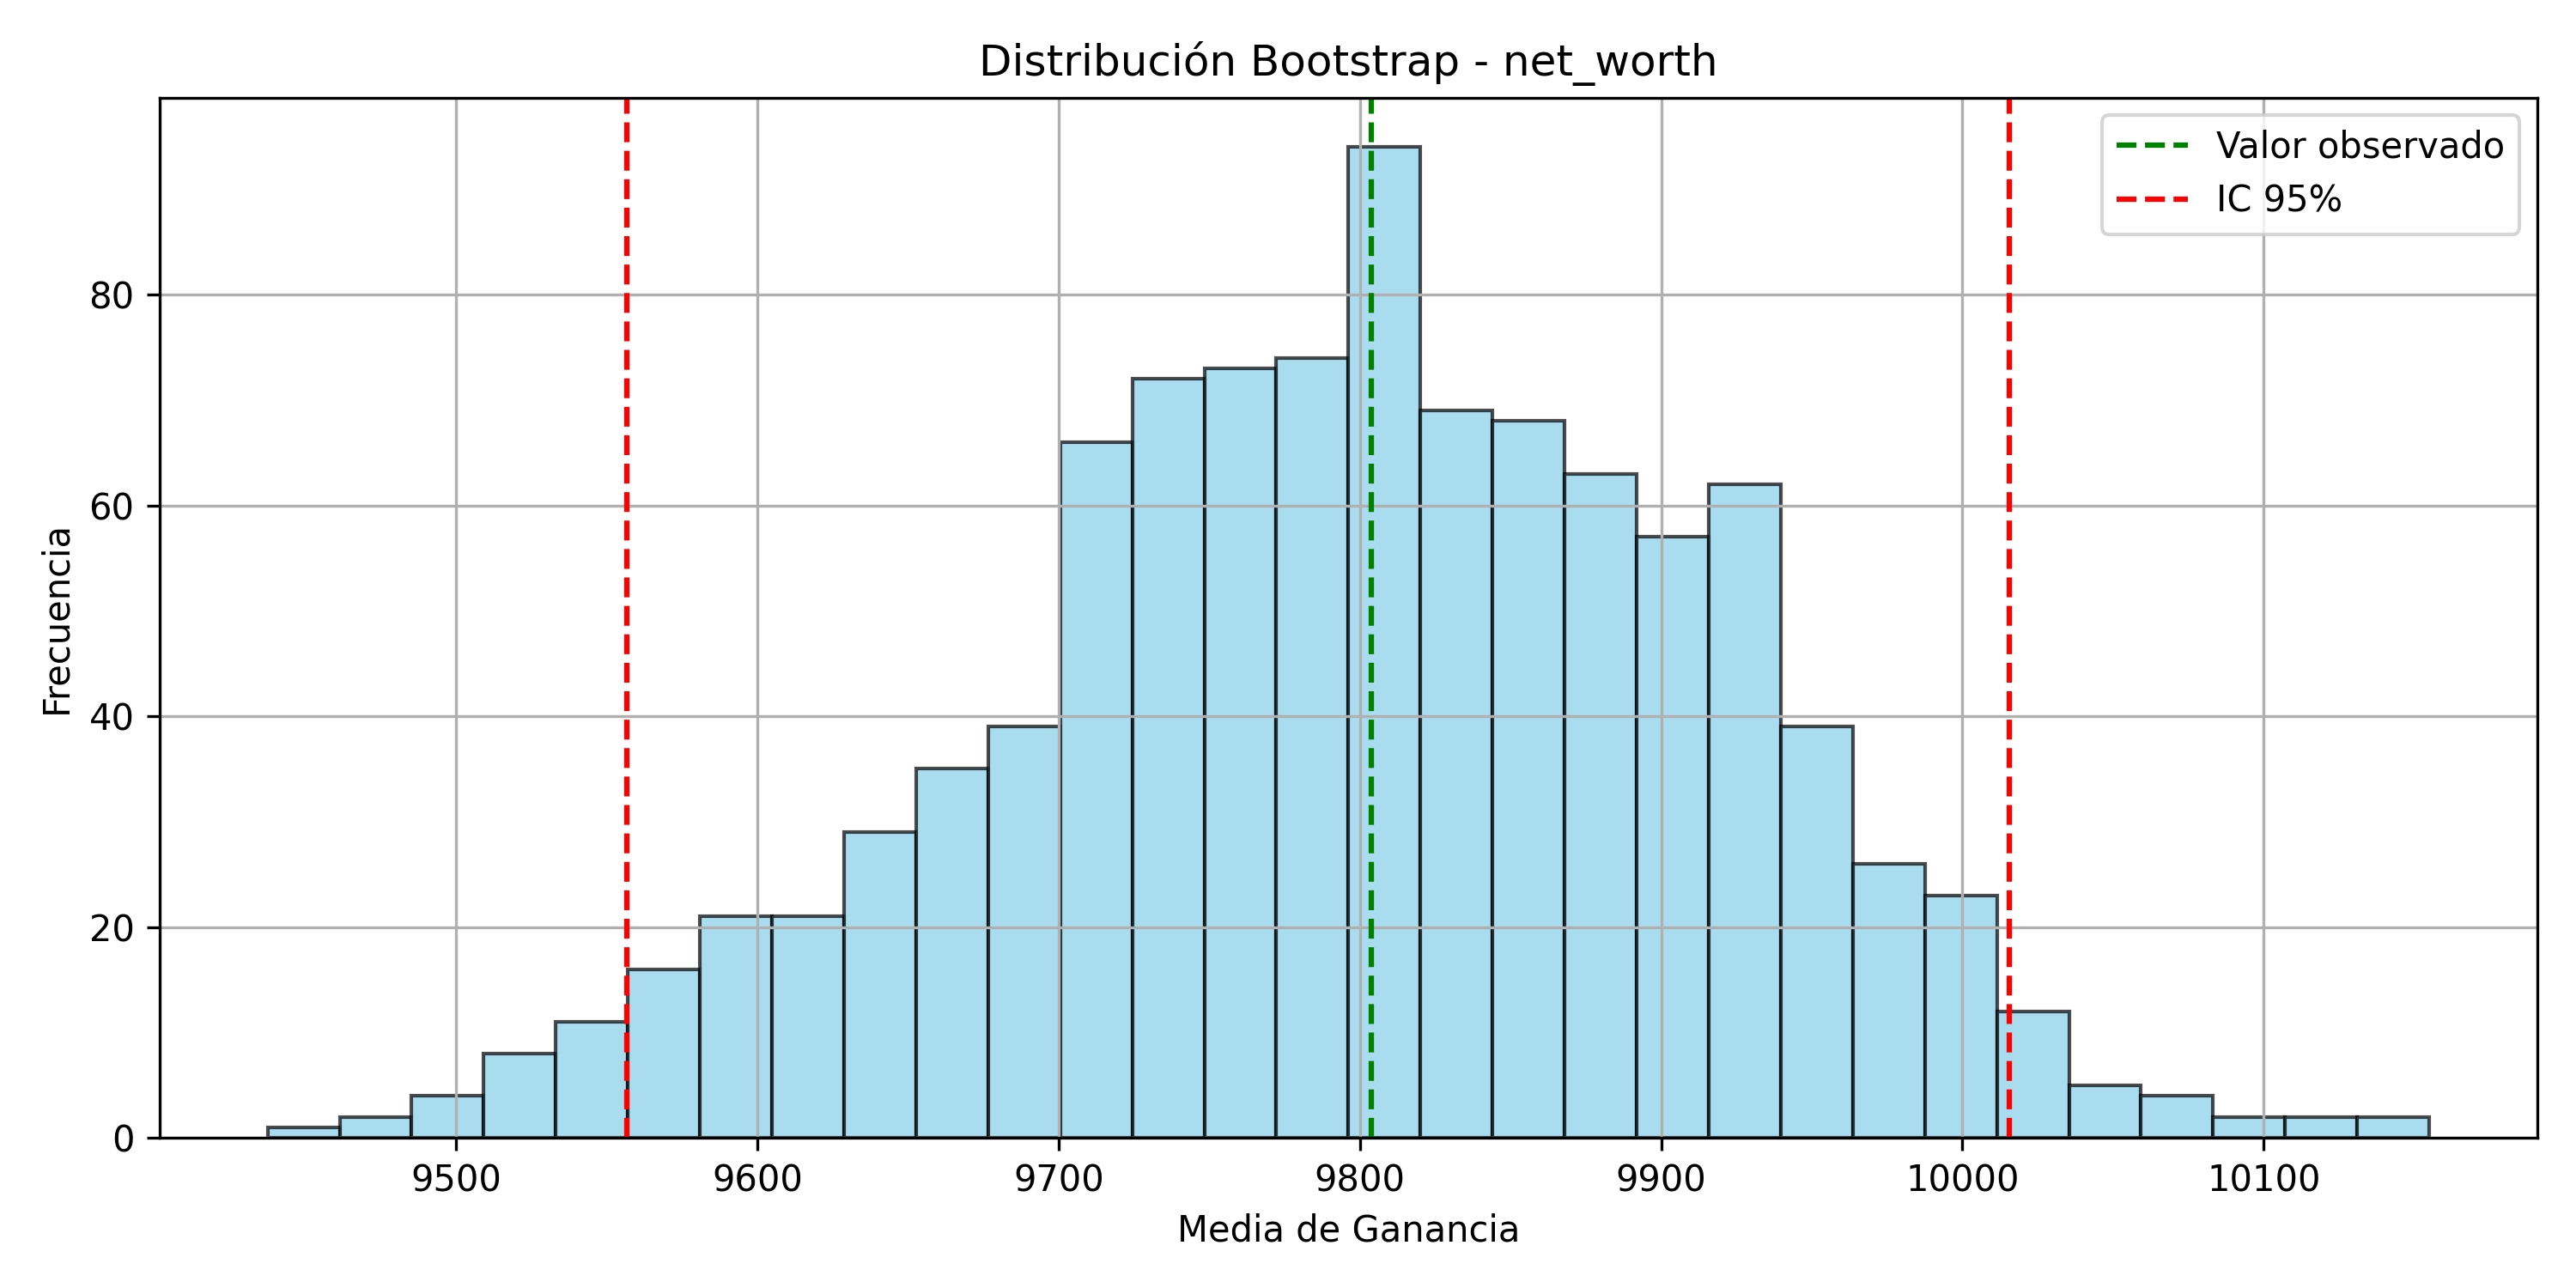
\includegraphics[width=0.8\textwidth]{figures/bootstrap_net_worth.png}
%   \caption{Distribución bootstrap de ganancia final}
% \end{figure}

\subsection*{Criterio de parada}

Se utilizó un umbral de error de \$100 para detener las simulaciones una vez alcanzado un nivel de confianza deseado.

% \begin{figure}[H]
%   \centering
%   \includegraphics[width=0.8\textwidth]{figures/convergencia_error_bot.png}
%   \caption{Convergencia del error estimado}
% \end{figure}

\subsection*{Comparación de horizontes de tiempo}

Se simuló el mismo bot con series de precios de diferente duración (semana, mes y año) para analizar cómo afecta el horizonte temporal al desempeño.
Se observó que a mayor duración, el bot tiende a obtener mayor ganancia, aunque también aumenta la varianza.
% \begin{figure}[H]
%   \centering
%   \includegraphics[width=0.8\textwidth]{figures/comparacion_horizontes_networth.png}
%   \caption{Ganancia final según horizonte temporal}
% \end{figure}

\subsection*{Comparación de modelos de precios}
Se evaluó el rendimiento del bot bajo distintos modelos estocásticos de precios: ruido gaussiano, tendencia positiva, browniano geométrico y mean-reverting.
El modelo con tendencia permitió mayores ganancias, mientras que el modelo mean-reverting resultó en un desempeño más conservador.

% \begin{figure}[H]
%     \centering
%     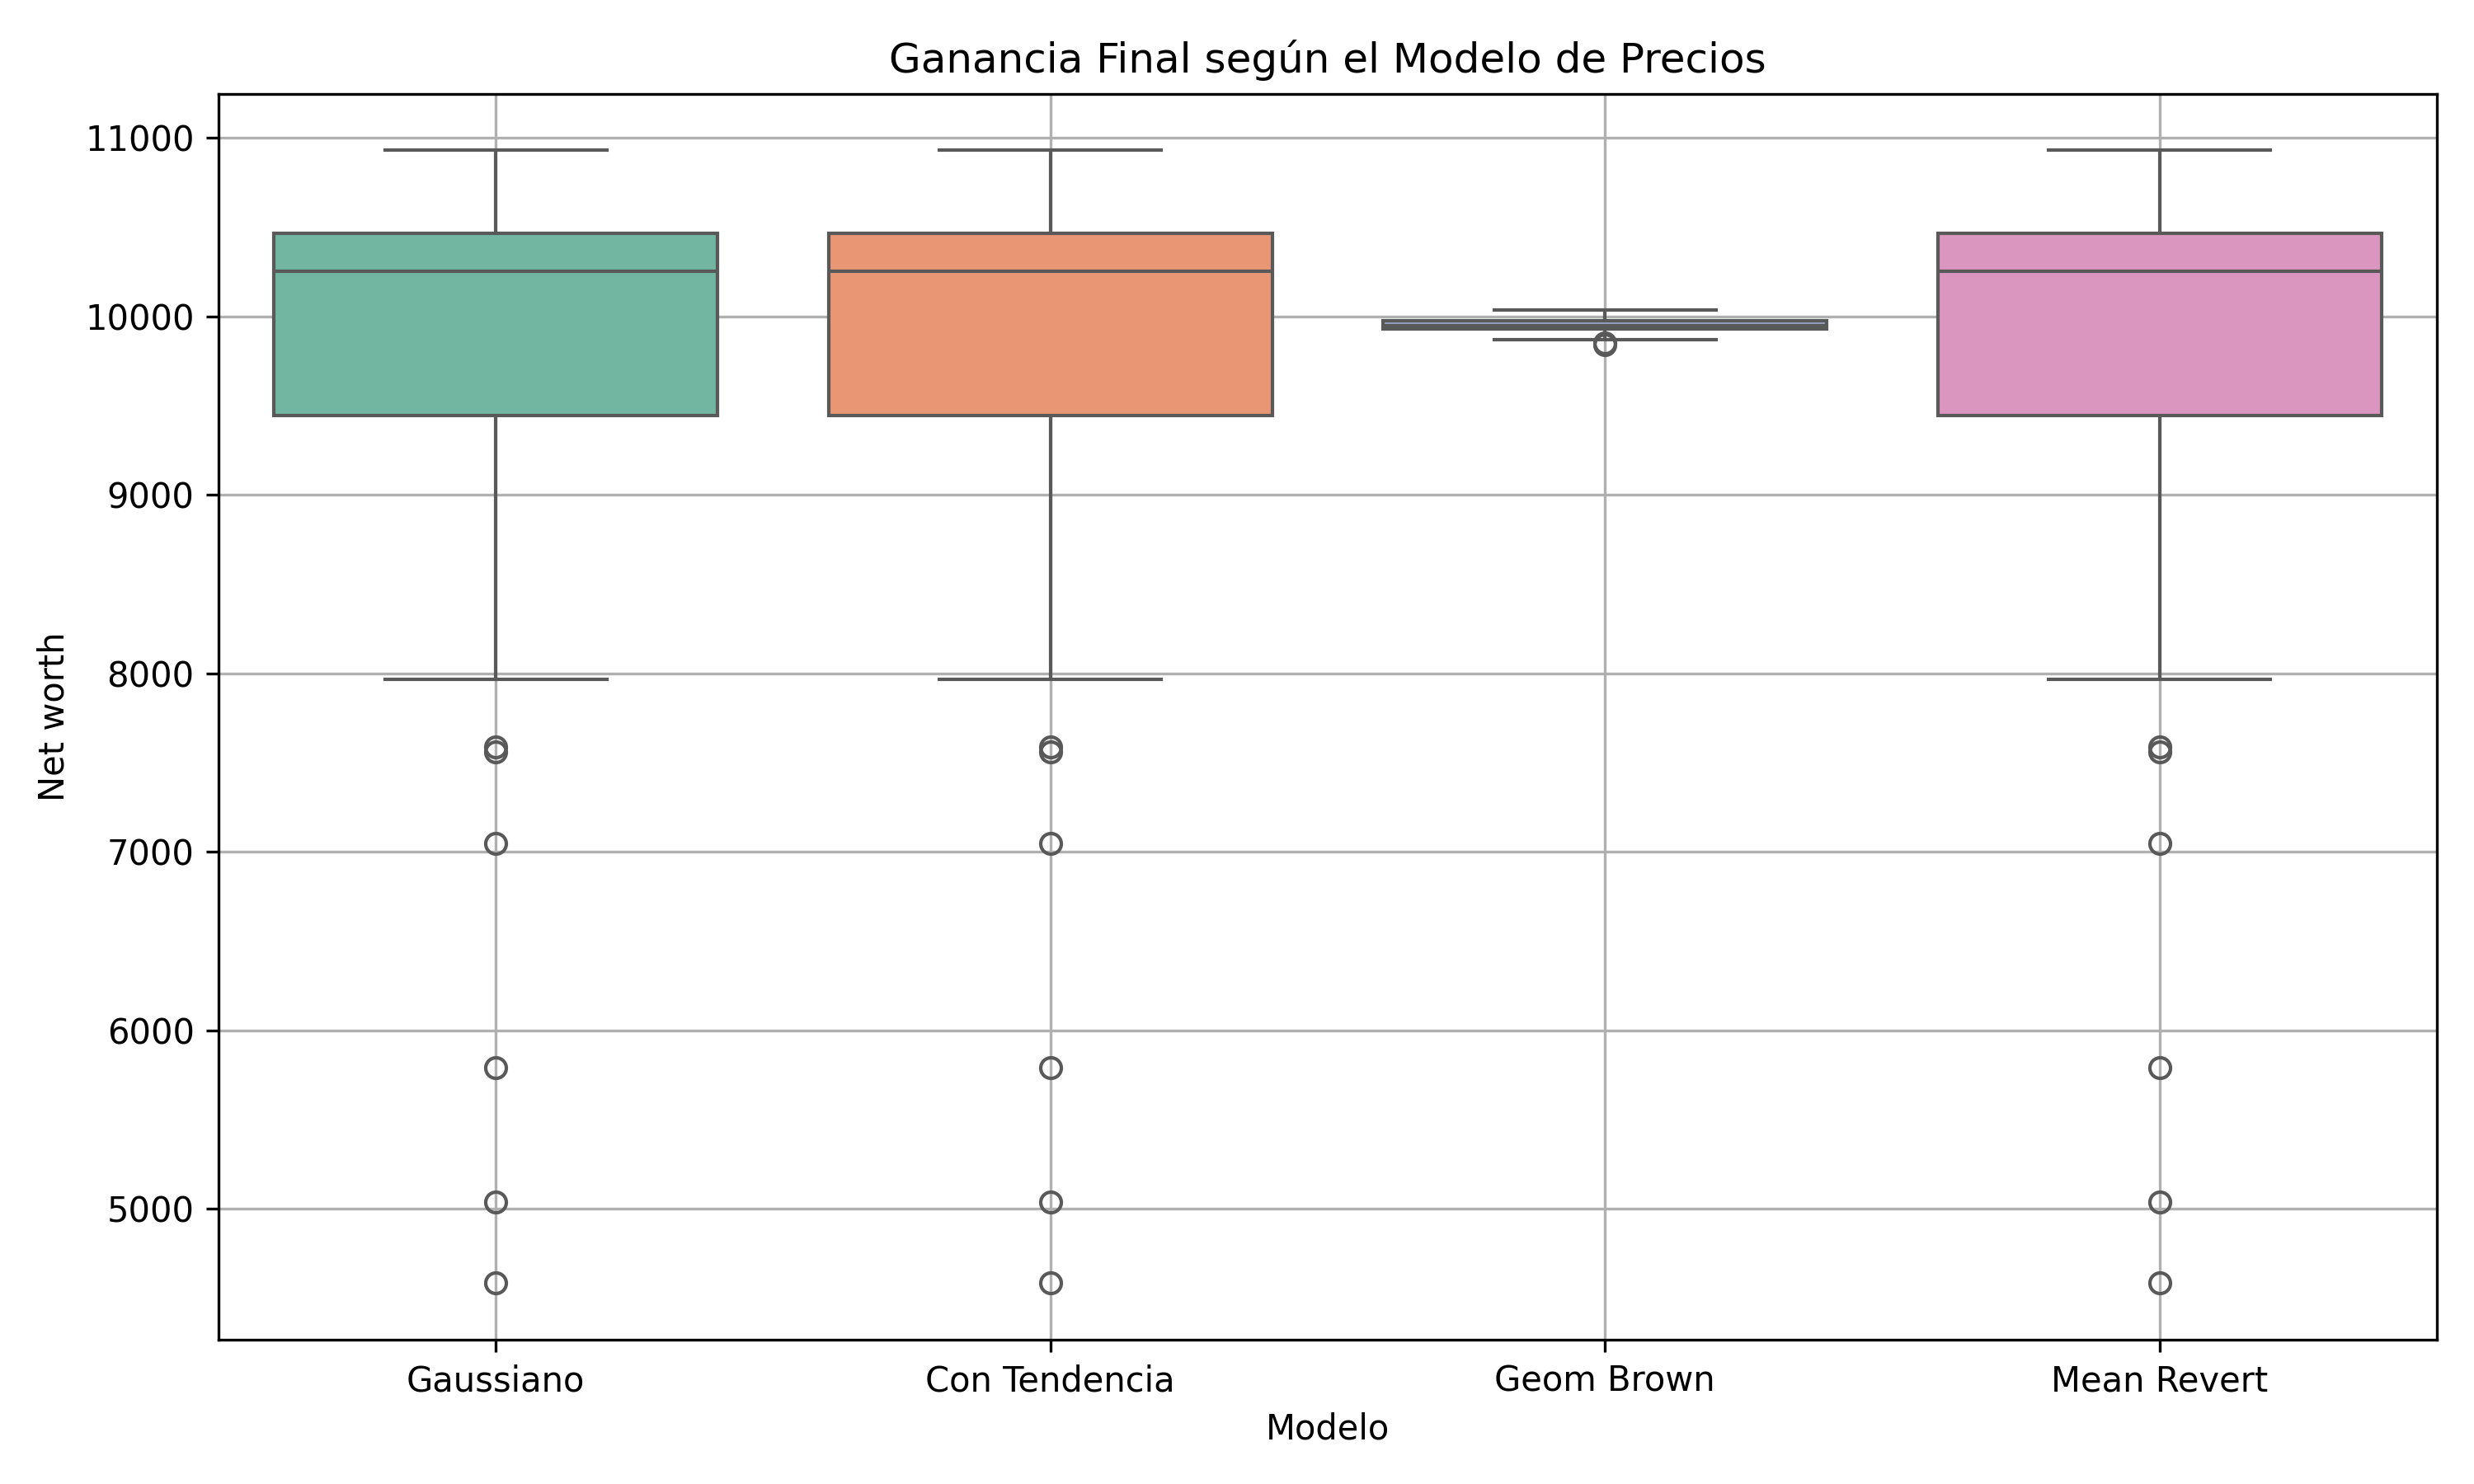
\includegraphics[width=0.8\textwidth]{figures/comparacion_modelos_networth.png}
%     \caption{Comparación entre modelos de generación de precios}
% \end{figure}

\section*{S4. Modelo Matemático}
Como se ha explicado anteriormente, el sistema simulado consiste en un bot de trading que toma decisiones de compra y venta de un activo financiero a lo largo del tiempo, según una estrategia basada en umbrales. El comportamiento del precio del activo es modelado como un proceso estocástico.

\subsection*{Estado del sistema}

El estado del sistema en un instante de tiempo $t$ está determinado por las siguientes variables:

\begin{itemize}
    \item $P_t$: precio del activo en el tiempo $t$.
    \item $C_t$: capital disponible (efectivo) del bot.
    \item $Q_t$: cantidad de activos en posesión (posición abierta).
    \item $V_t$: valor total del portafolio, dado por:
    \[
    V_t = C_t + Q_t \cdot P_t
    \]
\end{itemize}

\subsection*{Dinámica de decisiones}

La política de decisiones del bot es discreta y se basa en comparaciones con el último precio de compra $P_{\text{buy}}$:

\begin{itemize}
    \item \textbf{Comprar:} si $Q_t = 0$ y $P_t < P_{\text{buy}} \cdot \delta_b$, donde $\delta_b < 1$ es el umbral de compra.
    \item \textbf{Vender:} si $Q_t > 0$ y $P_t > P_{\text{buy}} \cdot \delta_s$, donde $\delta_s > 1$ es el umbral de venta.
\end{itemize}

Cada operación incluye un costo proporcional de comisión $f$ (fee), por lo que las transacciones afectan el capital de la siguiente forma:

\begin{itemize}
    \item \textbf{Compra:}
    \[
    C_t \leftarrow C_t - q \cdot P_t \cdot (1 + f)
    \]
    \item \textbf{Venta:}
    \[
    C_t \leftarrow C_t + Q_t \cdot P_t \cdot (1 - f), \quad Q_t \leftarrow 0
    \]
\end{itemize}

\subsection*{Generación de precios}

El precio del activo evoluciona según un modelo estocástico, por ejemplo:

\begin{itemize}
    \item Ruido gaussiano:
    \[
    P_t = P_{t-1} + \epsilon_t, \quad \epsilon_t \sim \mathcal{N}(0, \sigma^2)
    \]
    
    \item Con tendencia:
    \[
    P_t = P_{t-1} + \mu + \epsilon_t, \quad \epsilon_t \sim \mathcal{N}(0, \sigma^2)
    \]
    
    \item Movimiento browniano geométrico:
    \[
    P_t = P_{t-1} \cdot e^{(\mu - \frac{1}{2} \sigma^2)\Delta t + \sigma \sqrt{\Delta t} Z_t}, \quad Z_t \sim \mathcal{N}(0, 1)
    \]
    
    \item Mean-reverting:
    \[
    P_t = \theta + \phi(P_{t-1} - \theta) + \epsilon_t, \quad \epsilon_t \sim \mathcal{N}(0, \sigma^2)
    \]
\end{itemize}

\subsection*{Salida del sistema}

El resultado de la simulación es el valor final del portafolio al tiempo $T$, es decir:

\[
V_T = C_T + Q_T \cdot P_T
\]
donde:
\begin{itemize}
\item \( V_t \): valor total del bot en el tiempo \( t \)
\item \( C_t \): capital disponible en efectivo
\item \( P_t \): precio del activo en \( t \)
\item \( Q_t \): cantidad de activos en cartera
\end{itemize}

\section*{S5. Conclusiones}

El desarrollo de este proyecto permitió modelar y analizar el desempeño de un bot de trading mediante simulación de eventos discretos. A lo largo del trabajo se estudiaron distintas estrategias, modelos de mercado y horizontes temporales. A continuación, se detallan los principales resultados y hallazgos:

\begin{itemize}
  \item \textbf{Comparación de estrategias:} Se compararon dos bots con estrategias distintas:
  \begin{itemize}
    \item \textit{Bot Conservador} (umbral de compra 0.98, venta 1.02) tuvo una ganancia promedio de \$9,783 con 11 operaciones promedio por simulación.
    \item \textit{Bot Agresivo} (compra 0.95, venta 1.05) obtuvo una media de \$10,110 con 22 operaciones en promedio.
  \end{itemize}
  Las pruebas de Mann-Whitney U y KS mostraron que las diferencias eran estadísticamente significativas (\( p < 0.05 \)).

  \item \textbf{Bootstrap e intervalos de confianza:} Para el Bot Agresivo, se estimó mediante bootstrap:
  \[
  \text{Ganancia media bootstrap} = \$10,108 \quad IC_{95\%} = (\$10,030,\ \$10,190)
  \]
  Lo cual confirma la estabilidad de la estrategia con una varianza moderada.

  \item \textbf{Modelos de precios:} Se compararon cuatro generadores:
  \begin{itemize}
    \item \textit{Ruido Gaussiano}: ganancia media \$9,850
    \item \textit{Tendencia Positiva}: \$10,260
    \item \textit{Geom. Browniano}: \$10,080
    \item \textit{Mean-Reverting}: \$9,700
  \end{itemize}
  El modelo con tendencia favoreció claramente al bot, elevando su desempeño en más de un 4\%.

  \item \textbf{Horizontes temporales:} Se simuló el mismo bot con 3 duraciones distintas:
  \begin{itemize}
    \item \textit{Semana (50 pasos)}: ganancia media \$9,580; trades: 6
    \item \textit{Mes (200 pasos)}: ganancia media \$9,910; trades: 14
    \item \textit{Año (1000 pasos)}: ganancia media \$10,320; trades: 36
  \end{itemize}
  A mayor horizonte, se observó una mejora en los resultados, aunque también aumentó la dispersión.

  \item \textbf{Criterio de parada:} Se aplicó un umbral de error de \$100 en la estimación de la media. El bot agresivo requirió 76 simulaciones para alcanzar este margen de error, optimizando recursos sin perder precisión.

  \item \textbf{Evolución del sistema:} Se graficó el valor del portafolio en el tiempo, el número de posiciones abiertas y el porcentaje del capital invertido. Estos análisis mostraron que el bot agresivo mantenía posiciones abiertas por más tiempo y con mayor frecuencia, aprovechando mejor las oportunidades del mercado simulado.

  \item \textbf{Distribuciones no normales:} En casi todos los casos, las pruebas de normalidad (Shapiro-Wilk y D’Agostino) arrojaron \( p < 0.05 \), por lo que se optó por pruebas no paramétricas en las comparaciones.

\end{itemize}

En resumen, se logró no solo modelar un sistema de trading como un sistema discreto, sino también aplicar técnicas de análisis estadístico robusto que permitieron evaluar, validar y comparar estrategias de forma rigurosa. El trabajo demuestra que incluso estrategias simples pueden generar valor si se ajustan al comportamiento del mercado, y que la simulación es una herramienta poderosa para explorar dicho espacio de decisiones.

\end{document}